\subsection{Time-inhomogeneous processes}
\label{m:sec:inhomog}

In every chain defined so far the rates are fixed numbers. Several later
chapters need rates that vary with the clock: an environment that deteriorates,
a resource that depletes, a speciation rate that declines as the available
niche fills. This section sets up the time-inhomogeneous framework and works
through the standard example, the logistic speciation model, which is exactly
soluble at the level required here.

\subsubsection{Chains with time-dependent rates}
\label{m:sec:timedep}

A \emph{time-inhomogeneous} continuous-time Markov chain keeps the Markov
property \cref{m:eq:markov} but allows the transition rates to depend on
absolute time: in place of \cref{m:eq:infinitesimal},
\begin{equation}
\label{m:eq:infinitesimalt}
\pr{X_{t+\Delta t} = j \mid X_t = i} = q_{ij}(t)\,\Delta t + o(\Delta t)
\qquad (j\neq i) .
\end{equation}
The forward equations acquire a time-dependent generator,
\begin{equation}
\label{m:eq:timedepkolm}
\dda{P}{t} = P\,Q(t),
\qquad
\ddt{p_j(t)} = \sum_{k\neq j}q_{kj}(t)\,p_k(t) - q_j(t)\,p_j(t) ,
\end{equation}
and the holding time in state $i$ entered at time $s$ is no longer exponential
with a constant rate but has survival function
$\exp\bigl(-\int_s^t q_i(u)\,\dd u\bigr)$. Two structural losses should be
noted. The transition probabilities no longer form a semigroup --- they depend
on the starting time as well as the elapsed time --- and there is in general no
stationary distribution to converge to, because the target itself is moving.
What survives, and this is what the methods of \cref{m:sec:methct} exploit, is
linearity: \cref{m:eq:timedepkolm} is still a linear system, generating
functions still convert it to a first-order equation, and first-step arguments
still close, now with $t$-dependent coefficients.

\subsubsection{The time-inhomogeneous linear birth--death process}
\label{m:sec:tibd}

The linear birth--death process with rates $\lambda(t)$, $\mu(t)$ --- each
individual gives birth at rate $\lambda(t)$ and dies at rate $\mu(t)$, the
rates being prescribed functions of time --- is the workhorse example. The
master equation is \cref{m:eq:bdmaster} with $t$-dependent coefficients, and
the generating function satisfies
\begin{equation}
\label{m:eq:tibdpde}
\pddt{G} = \bigl(\lambda(t) z^2 - (\lambda(t)+\mu(t))z + \mu(t)\bigr)\pdd{G}{z}.
\end{equation}
Two quantities remain explicit for arbitrary integrable rates. The mean, by the
same conditioning argument as in the homogeneous case, solves
$\ddt{\ex{X_t}} = (\lambda(t)-\mu(t))\ex{X_t}$, hence
\begin{equation}
\label{m:eq:meanodeinhom}
\ex{X_t} = N\exp\lrb{\int_0^t\bigl(\lambda(s)-\mu(s)\bigr)\dd s} .
\end{equation}
The extinction probability $u(t)=\pr{X_t=0}$, started from one individual,
solves the Riccati equation
\begin{equation}
\label{m:eq:riccatiext}
\dda{u}{t} = \mu(t) - \bigl(\lambda(t)+\mu(t)\bigr)u + \lambda(t)u^2,
\qquad u(0) = 0 ,
\end{equation}
which is the backward equation of \cref{m:sec:backward} with time-dependent
coefficients: in the first small interval either a death occurs, contributing
$\mu(t)\Delta t$, or a birth occurs, contributing
$\lambda(t)\Delta t\,u(t)^2$ since both daughter lineages must then die out,
or nothing occurs. The full generating function retains the fractional-linear
form of \cref{m:eq:bdsolution}, with constant coefficients replaced by
solutions of the same Riccati equation; when \cref{m:eq:riccatiext} cannot be
solved in closed form, it is at least a scalar equation and is integrated
numerically without difficulty.

\subsubsection{The logistic speciation model}
\label{m:sec:logspec}

The standard macroevolutionary application of \cref{m:sec:tibd} lets the
speciation rate decline with diversity \cite{Allen2010}. Let $X_t$ count
species, each of which speciates at rate
\begin{equation}
\label{m:eq:speciationrate}
\lambda(n) = \lambda_0\lrb{1-\frac{n}{K}}
\end{equation}
when the standing diversity is $n$, and goes extinct at constant rate $\mu$,
with $\lambda_0>\mu$ and $K$ the niche capacity. The chain with the genuinely
state-dependent rate \cref{m:eq:speciationrate} is nonlinear and has no closed
solution; the standard tractable surrogate replaces the random diversity in
\cref{m:eq:speciationrate} by the deterministic mean-field trajectory, yielding
a \emph{time-inhomogeneous} linear process in the sense of \cref{m:sec:tibd}.
The substitution is a modelling step, not an identity, and is flagged as such
wherever the model is used below.

The mean-field diversity $\bar N(t)$ solves
\begin{equation}
\label{m:eq:logisticode}
\dda{\bar N}{t} = \bigl(\lambda(\bar N)-\mu\bigr)\bar N
= r\bar N\lrb{1-\frac{\bar N}{N_\ast}},
\qquad
r = \lambda_0-\mu,
\quad
N_\ast = K\lrb{1-\frac{\mu}{\lambda_0}},
\end{equation}
the logistic equation, whose carrying point $N_\ast$ is the diversity at which
speciation balances extinction. Starting from $\bar N(0)=N_0$,
\begin{equation}
\label{m:eq:logisticsol}
\bar N(t) = \frac{N_\ast}{1+B\ee^{-rt}},
\qquad B = \frac{N_\ast}{N_0}-1 ,
\end{equation}
and the surrogate speciation rate $\lambda(t)=\lambda_0(1-\bar N(t)/K)$ is
\begin{equation}
\label{m:eq:lambdat}
\lambda(t) = \mu + \frac{rB\ee^{-rt}}{1+B\ee^{-rt}},
\qquad
\lambda(0) = \lambda_0\lrb{1-\frac{N_0}{K}},
\end{equation}
relaxing monotonically from $\lambda(0)$ down to $\mu$
(\cref{m:fig:logspec}). The accumulated net growth needed in
\cref{m:eq:meanodeinhom} evaluates in closed form,
\begin{equation}
\label{m:eq:lambdaint}
\int_0^t\bigl(\lambda(s)-\mu\bigr)\dd s
= \ln\lrb{\frac{1+B}{1+B\ee^{-rt}}},
\end{equation}
so the mean diversity of the surrogate process is
\begin{equation}
\label{m:eq:logspecmean}
\ex{X_t} = N_0\,\frac{1+B}{1+B\ee^{-rt}}
\;\xrightarrow[t\to\infty]{}\;
N_0(1+B) = N_\ast ,
\end{equation}
which recovers the deterministic equilibrium, as a linear mean-field surrogate
should. Its extinction probability is obtained by integrating
\cref{m:eq:riccatiext} with the rate \cref{m:eq:lambdat}. Two limiting
behaviours are worth noting: at early times $\lambda(t)\approx\lambda(0)$ and
the process is indistinguishable from a homogeneous supercritical one, while at
late times $\lambda(t)\to\mu$ from above and the chain approaches criticality
--- the regime whose discrete-generation difficulties are documented in
\cref{m:app:critical}.

\begin{figure}[ht]
\centering
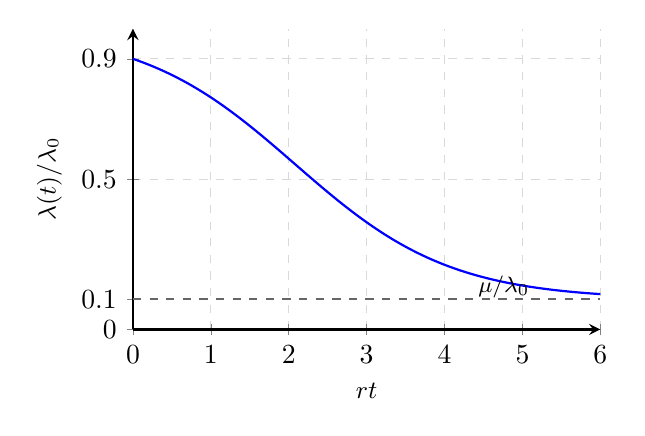
\begin{tikzpicture}
\begin{axis}[
    width=0.62\textwidth, height=5.4cm,
    axis lines=left,
    xlabel={$rt$}, ylabel={$\lambda(t)/\lambda_0$},
    xmin=0, xmax=6, ymin=0, ymax=1.0,
    xtick={0,1,2,3,4,5,6}, ytick={0,0.1,0.5,0.9},
    grid=major, grid style={dashed, gray!30}, thick,
    label style={font=\small}
]
\addplot[blue, thick, domain=0:6, samples=120] {(0.1+8*exp(-x))/(1+8*exp(-x))};
\draw[dashed, black!60] (axis cs:0,0.1) -- (axis cs:6,0.1);
\node[font=\footnotesize, anchor=west] at (axis cs:4.3,0.14) {$\mu/\lambda_0$};
\end{axis}
\end{tikzpicture}
\caption{The diversity-dependent speciation rate \cref{m:eq:lambdat} of the
logistic speciation model, in units of $\lambda_0$ and against the rescaled
time $rt$, for $\mu/\lambda_0=0.1$ and $N_\ast/N_0=9$ (so $B=8$ and
$\lambda(0)=0.9\lambda_0$). The rate relaxes from $\lambda(0)$ down to the
extinction rate $\mu$ as the mean-field diversity \cref{m:eq:logisticsol}
fills the equilibrium $N_\ast$; the integrated intensity
\cref{m:eq:lambdaint} controls the mean \cref{m:eq:logspecmean}.}
\label{m:fig:logspec}
\end{figure}

\begin{figure}[ht]
\centering

\includegraphics[width=0.86\textwidth]{figures/logspec_mean.pdf}
\caption{Mean diversity \cref{m:eq:logspecmean} of the logistic speciation
surrogate for $N_0=1,3,6$, with the chapter's parameters
$\mu/\lambda_0=0.1$, $K=10$ (so $N_\ast=9$), plotted against the rescaled time
$rt$. Every founding diversity relaxes monotonically to the equilibrium
$N_\ast=K(1-\mu/\lambda_0)$, and the mean trajectory coincides with the
deterministic mean-field solution \cref{m:eq:logisticsol} --- the surrogate is
linear, so its mean closes exactly. Small founding cohorts spend a long early
interval in near-exponential growth before the diversity dependence binds.}
\label{m:fig:logspecmean}
\end{figure}

\FloatBarrier
